\documentclass[tikz,border=5pt]{standalone}
\usepackage{tikz}
\usepackage{amsmath}
\usetikzlibrary{arrows.meta}
\definecolor{nebula}{HTML}{6366F1}
\definecolor{spark}{HTML}{14B8A6}
\definecolor{ink}{HTML}{334155}
\begin{document}
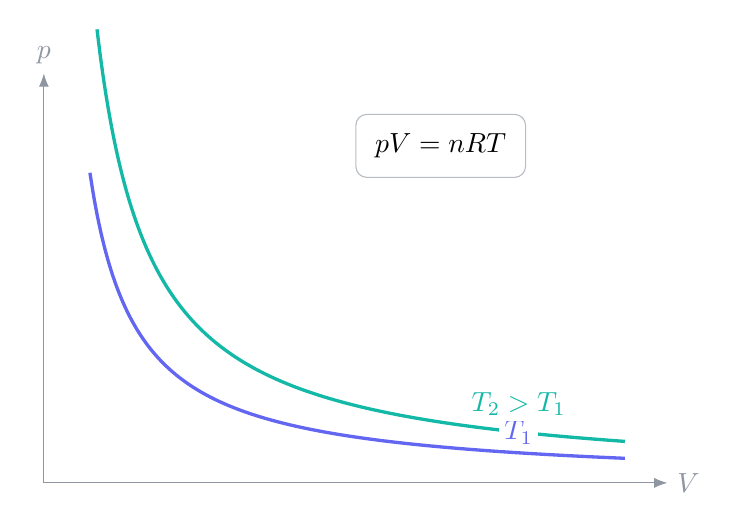
\begin{tikzpicture}[font=\sffamily,>=Latex,x=.9cm,y=.8cm]
  \draw[->,ink!55] (0,0)--(8.8,0) node[right] {$V$};
  \draw[->,ink!55] (0,0)--(0,6.5) node[above] {$p$};
  \draw[very thick,nebula,domain=.65:8.2,samples=150,smooth] plot(\x,{3.2/\x});
  \draw[very thick,spark,domain=.75:8.2,samples=150,smooth] plot(\x,{5.4/\x});
  \node[text=nebula,fill=white,inner sep=2pt] at (6.7,.8) {$T_1$};
  \node[text=spark,fill=white,inner sep=2pt] at (6.7,1.25) {$T_2>T_1$};
  \node[draw=ink!35,rounded corners=4pt,fill=white,inner sep=7pt] at (5.6,5.35)
    {$pV=nRT$};
\end{tikzpicture}
\end{document}
